\begin{frame}
  \begin{itemize}
    \item Find a way to measure how well a parametric model predicts known
      data (the training set).
    \item Use that information to adjust the
      parameters and make the model more accurate
    \item Repeat until a "good enough" model is found
  \end{itemize}
\end{frame}

\begin{frame}
  \frametitle{The error function}
  \begin{center}
    $e(w) = |h_w(x) - y|$ \\~\\
    "The error is 1 if the model is wrong, 0 if correct"
  \end{center}
\end{frame}


\begin{frame}
  \begin{center}
    $E(w) = \displaystyle\sum_{i = 1}^n{|h_w(x^{(i)}) - y^{(i)}|}$ \\~\\
    "Add 1 for every labeled data where the model is wrong"
  \end{center}
\end{frame}

\begin{frame}
  \frametitle{Error function}
  \begin{center}
    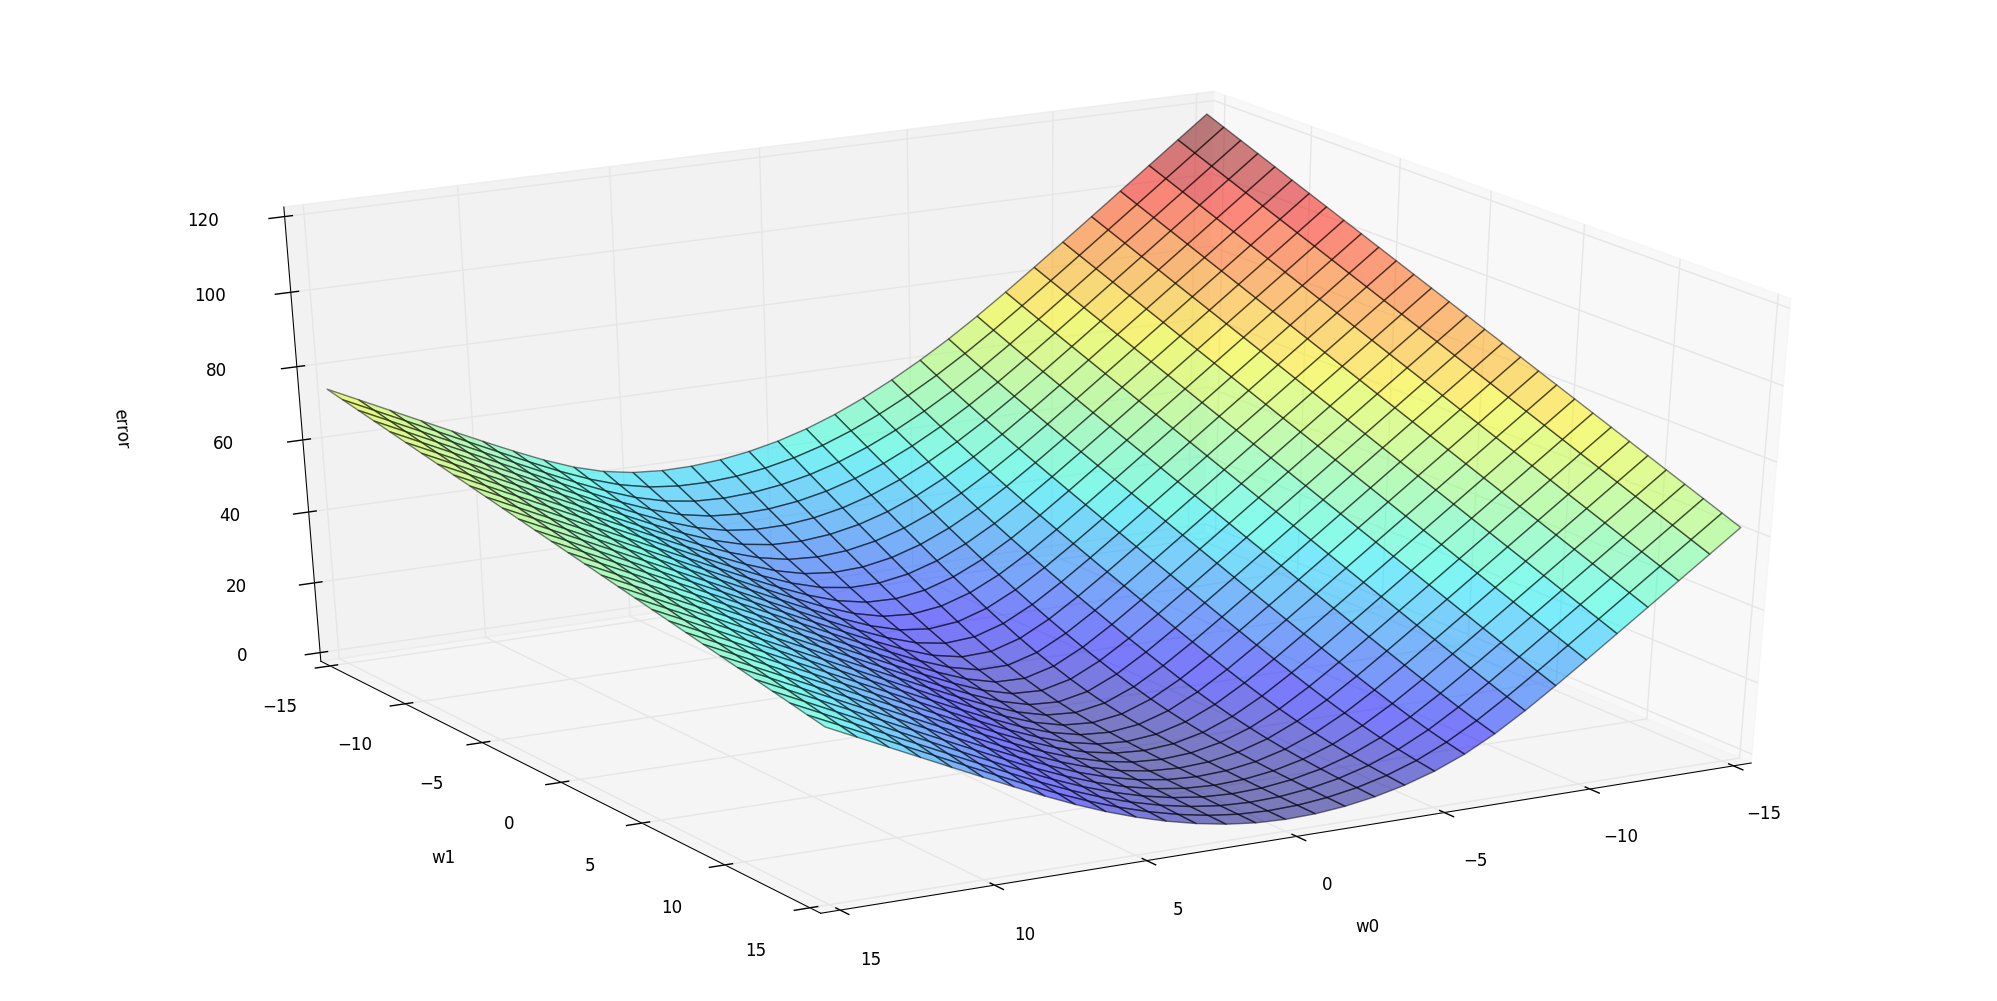
\includegraphics[scale=0.22]{./pictures/error_function.png}
  \end{center}
\end{frame}

\begin{frame}
  \frametitle{The logistic function}
  \begin{center}
    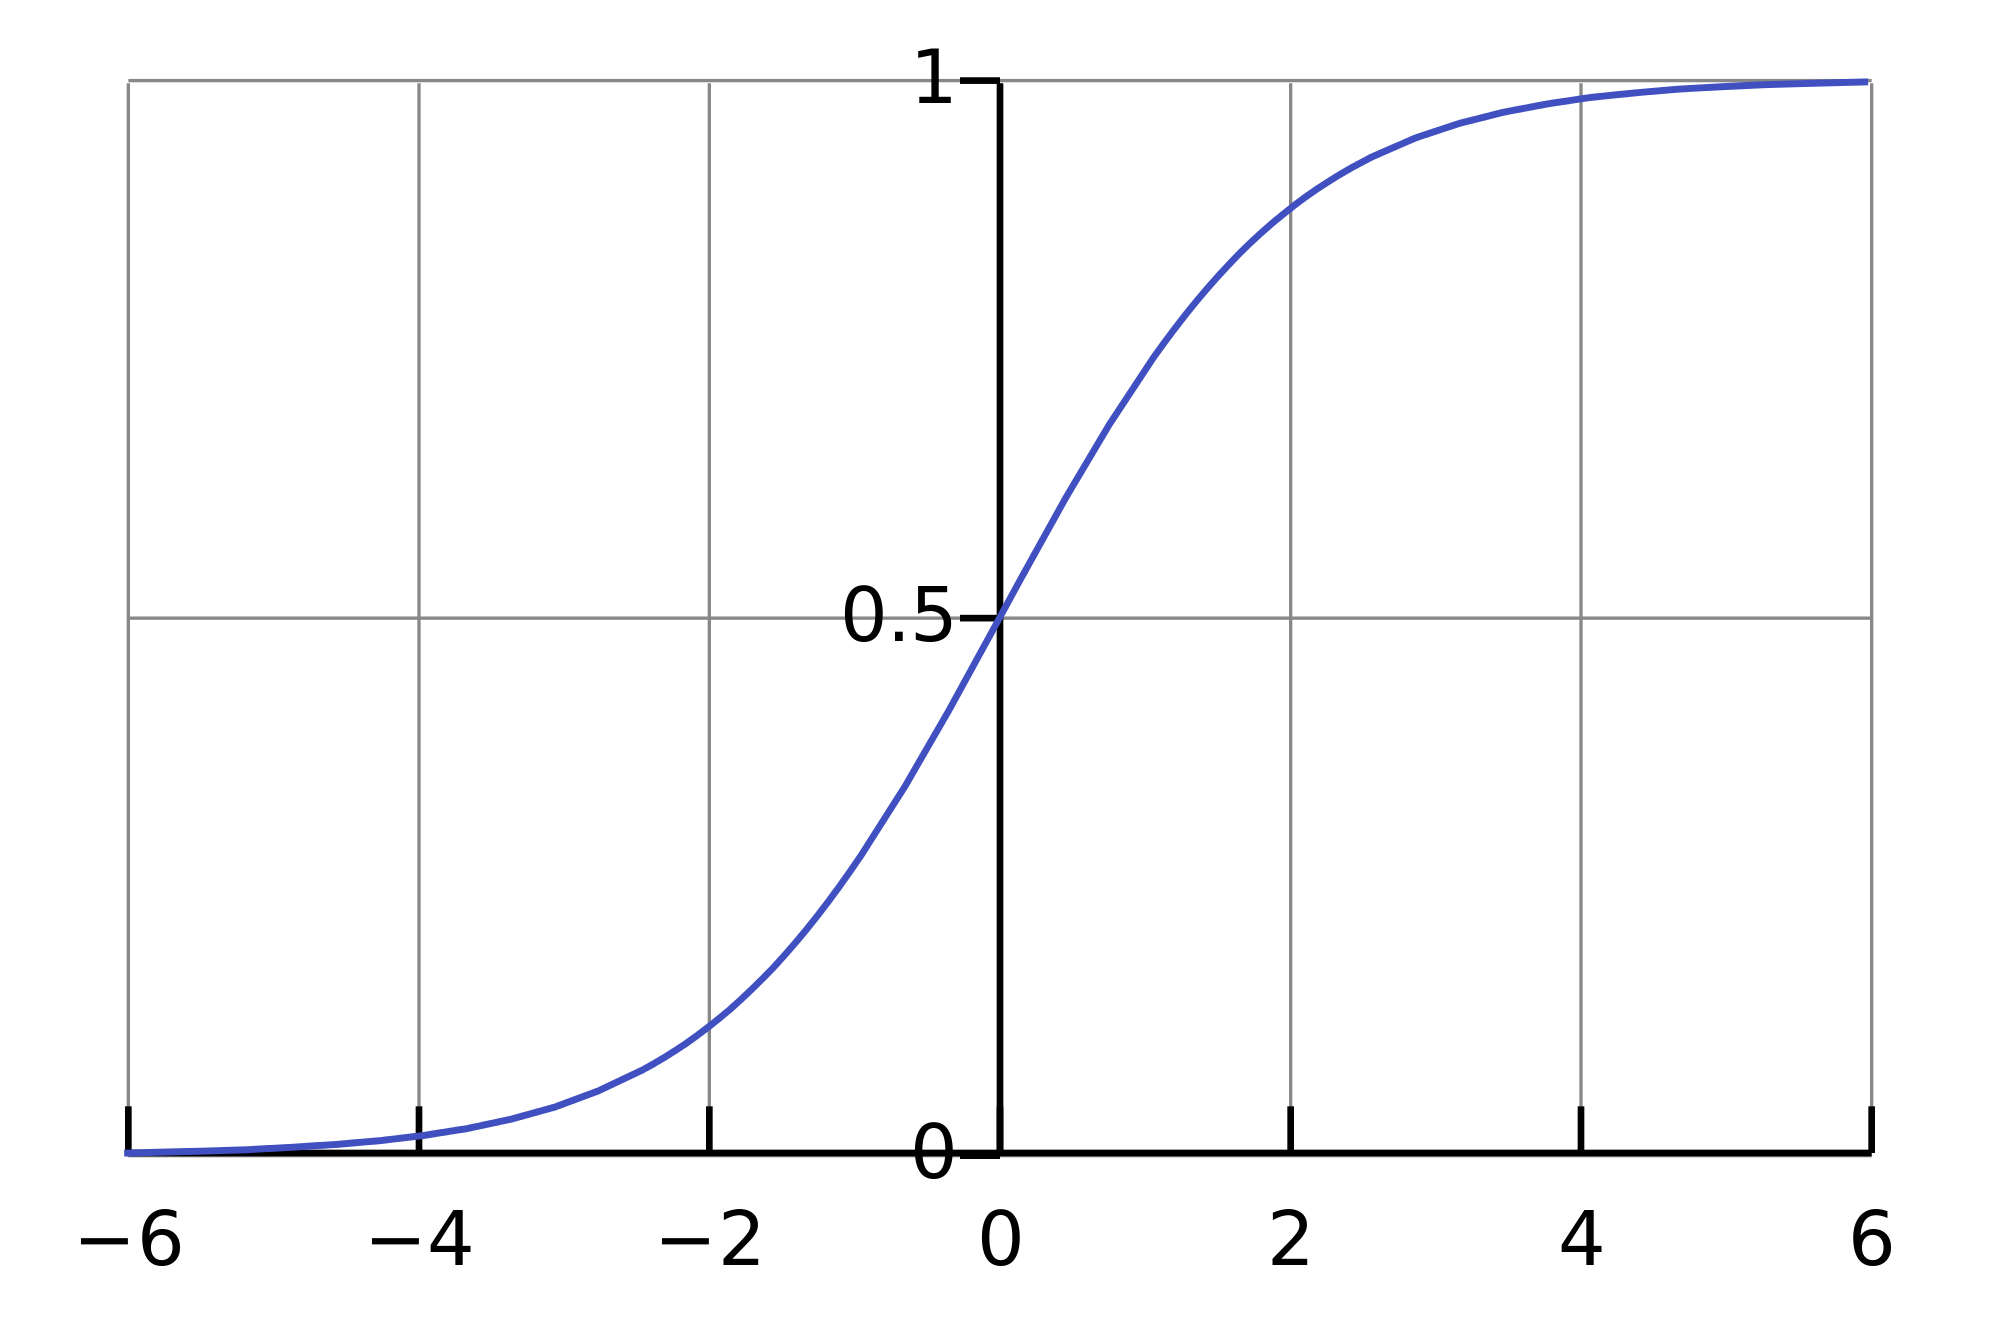
\includegraphics[scale=0.14]{./pictures/sigmoid.png}
  \end{center}
\end{frame}

\begin{frame}[fragile]
  \begin{block}{Logistic function}
    \begin{lstlisting}
      def g(x):
      1 / (1 + exp(-x))
    \end{lstlisting}
  \end{block}
\end{frame}

\begin{frame}
  \frametitle{Gradient descent}
  \begin{center}
    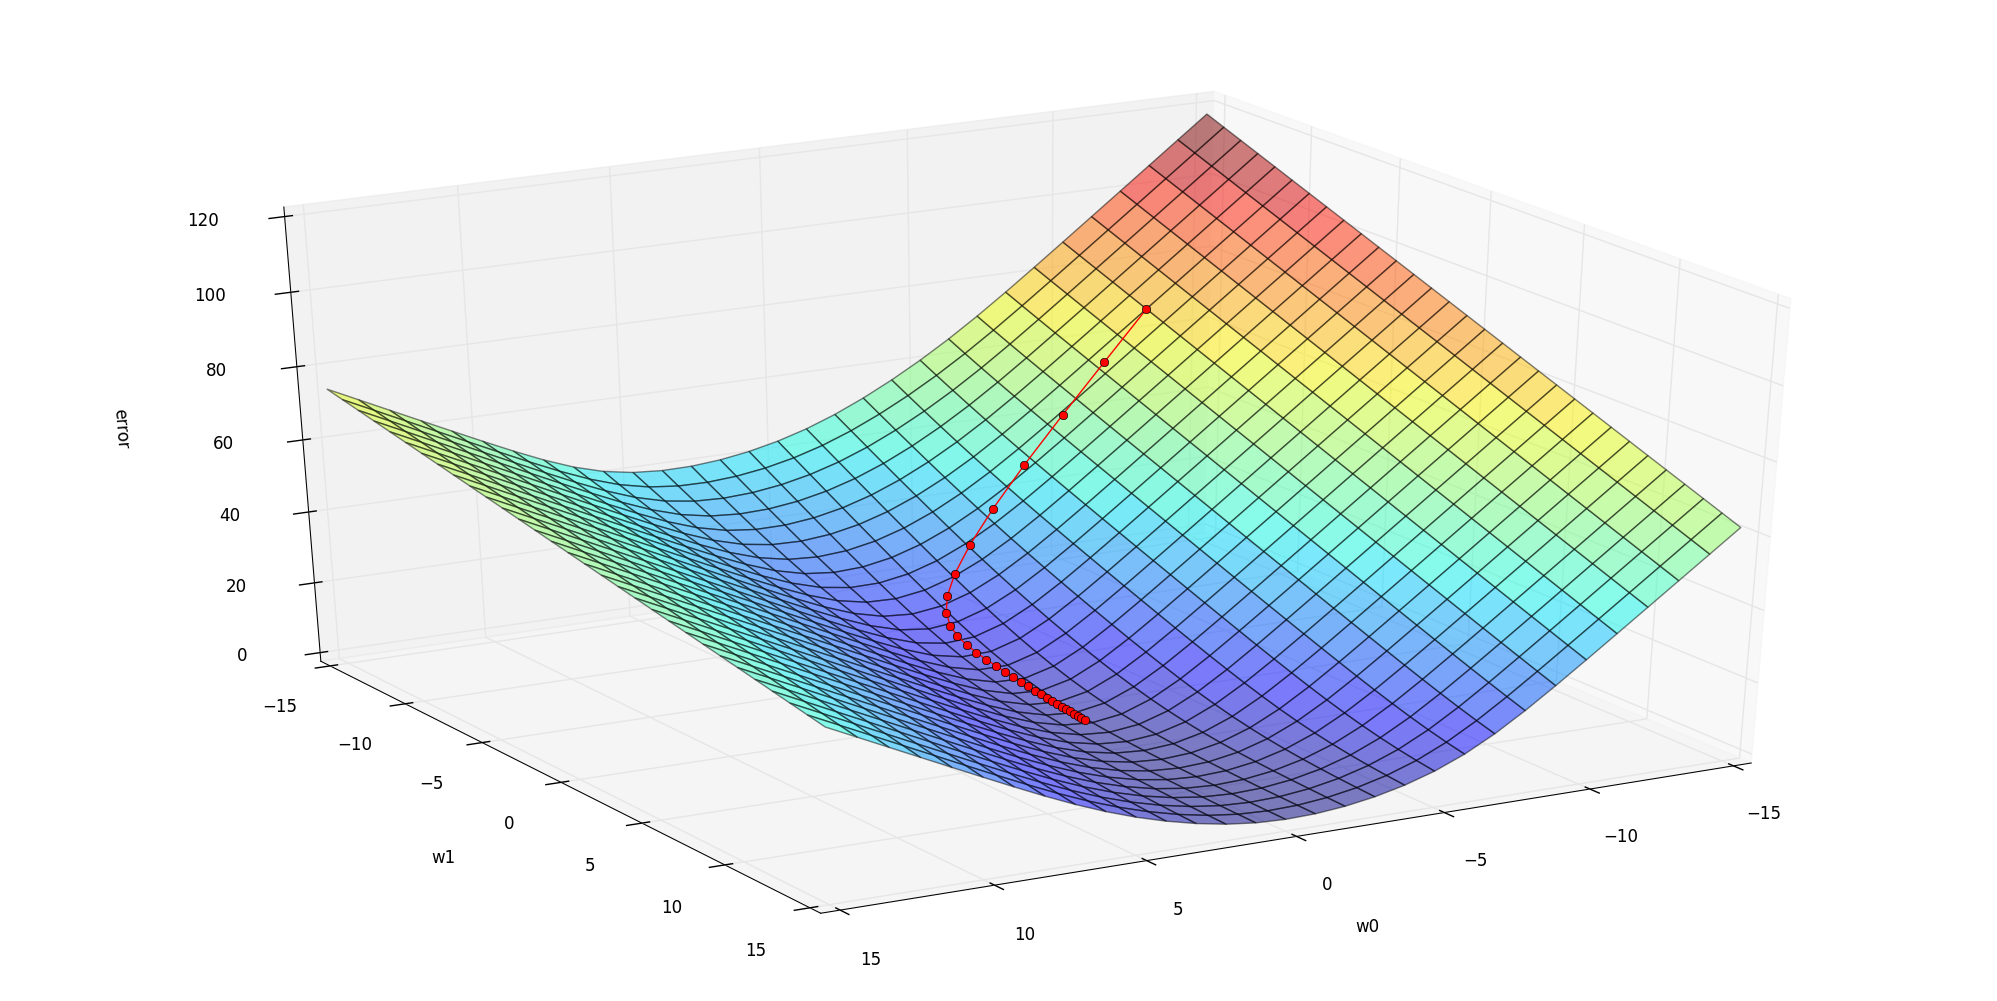
\includegraphics[scale=0.22]{./pictures/gradient_descent.png}
  \end{center}
\end{frame}
